\section{A Direct Ground-Truth Invalidation Witness}
\label{sec:direct}
Figure~\ref{fig:witness} reconstructs a released AWM Shopping trajectory under shuffle seed 42. Task 509 asks the agent to purchase a Cole Haan dress chukka boot. The agent reaches the checkout success page. The log records a \$464 subtotal with \$5 shipping, yielding a \$469 order. The benchmark scorer assigns FAIL with score 0, yet the completed checkout remains in the shopping backend.

Twenty-six minutes later, task 96 asks for the status of the latest order. The agent opens the account and reads Order \#000000197. The order is Pending and contains the same Cole Haan item with the same \$469 total. The agent reports this current state. Its evaluator still expects the earlier canceled order, so the task receives FAIL. Under the ordinal stream, task 96 occurs before the purchase tasks and all six AWM/ReasoningBank ordinal replications pass.

\begin{figure}[t]
\centering
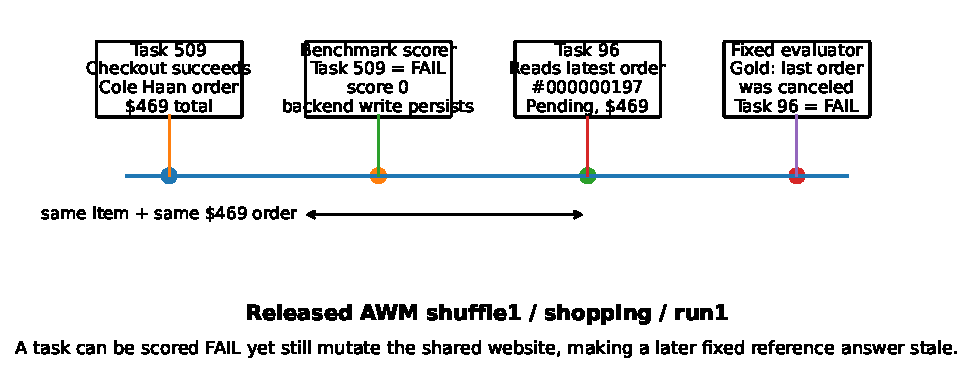
\includegraphics[width=\linewidth]{figures/fig2_direct_witness.pdf}
\caption{Direct released-trajectory witness. A scorer-failed purchase persists in the shopping backend. The downstream agent observes the resulting current order while the evaluator continues to score an earlier service state.}
\label{fig:witness}
\end{figure}

The witness establishes that benchmark score and environment mutation are separate state transitions. It also establishes that a current-state answer can be semantically correct while fixed reference text has become stale. This writer--reader chain supplies a direct mechanism for order-dependent evaluation error.

\section{Results}
\label{sec:results}

\subsection{Dynamic-reference failures replicate across methods and orders}
Figure~\ref{fig:sentinels} reports the three sentinels. Across AWM and ReasoningBank, every ordinal replicate passes: 18/18 method--run units. Across the two shuffled streams, none passes: 0/36. For each sentinel under each shuffle seed, all six paired method--run comparisons move from ordinal PASS to shuffled FAIL. The reverse transition never occurs. The two-sided exact sign test gives $p=0.03125$ for every six-pair panel.

Task 189 shows the same ground-truth shift at the value level. One AWM shuffle run identifies Order \#000000191 as the current latest pending order with total \$478.42. The fixed reference remains \$754.99.

Task 198 reproduces the mechanism on Shopping Admin. A shuffled run identifies Sarah Miller on the current most recent canceled order \#000000299. The fixed reference remains Lily Potter. Earlier shuffled tasks directly mutate the order database, so the changed reference object follows from the tested task stream itself.

\begin{figure}[t]
\centering
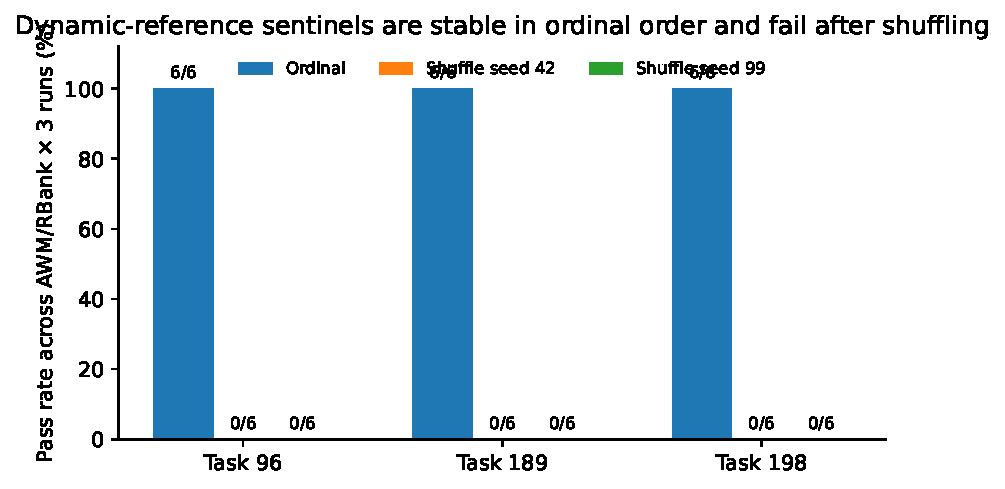
\includegraphics[width=0.96\linewidth]{figures/fig3_sentinel_replication.pdf}
\caption{Three dynamic-reference sentinels across AWM and ReasoningBank. Each bar aggregates three runs per method. All 18 ordinal units pass; all 36 shuffled units fail.}
\label{fig:sentinels}
\end{figure}

\subsection{State exposure is common in released shuffles}
Across the 48 shuffled memory-method run-domain cells in the four mutable single-site domains, the strict exposure detector identifies 887 state-sensitive reader units that follow at least one overlapping benchmark-successful writer. Of these units, 424 fail. Table~\ref{tab:exposure} shows the corresponding failure rates. Exposure becomes substantially more common under shuffling because mutating tasks move ahead of dynamic-reference queries.

\begin{table}[t]
\centering
\caption{Released-trajectory retrospective using the frozen writer--reader exposure rule.}
\label{tab:exposure}
\small
\begin{tabular}{llrrrr}
\toprule
Method & Order & Success & Exposed & Exp. fail & Clean fail \\
\midrule
AWM & ordinal & 56.43\% & 60 & 18.33\% & 33.33\% \\
AWM & seed 42 & 51.99\% & 227 & 49.78\% & 33.95\% \\
AWM & seed 99 & 51.30\% & 208 & 48.56\% & 37.50\% \\
ReasoningBank & ordinal & 59.73\% & 58 & 27.59\% & 31.30\% \\
ReasoningBank & seed 42 & 52.12\% & 224 & 45.98\% & 39.29\% \\
ReasoningBank & seed 99 & 52.32\% & 228 & 46.93\% & 38.89\% \\
\bottomrule
\end{tabular}
\end{table}

For AWM, exposed-reader failure reaches 49.78\% under seed 42 and 48.56\% under seed 99. The corresponding clean-reader rates are 33.95\% and 37.50\%. ReasoningBank shows the same direction: exposed-reader failure reaches 45.98\% and 46.93\%, compared with 39.29\% and 38.89\% for clean readers. The retrospective therefore connects the direct witness to a broader population of order-sensitive measurement objects.

\subsection{State-sensitive tasks account for a material part of the order gap}
Figure~\ref{fig:gap} compares the released ordinal-to-shuffle success gap with the same contrast after state-sensitive readers are excluded. For AWM, the raw gap is 4.44 percentage points under seed 42 and 5.13 points under seed 99. The filtered gaps are 2.46 and 3.36 points, corresponding to reductions of 44.5\% and 34.6\%.

ReasoningBank starts with raw gaps of 7.61 and 7.40 points. After the same exclusion, the gaps are 6.48 and 6.11 points. The reductions are 14.9\% and 17.5\%.

\begin{figure}[t]
\centering
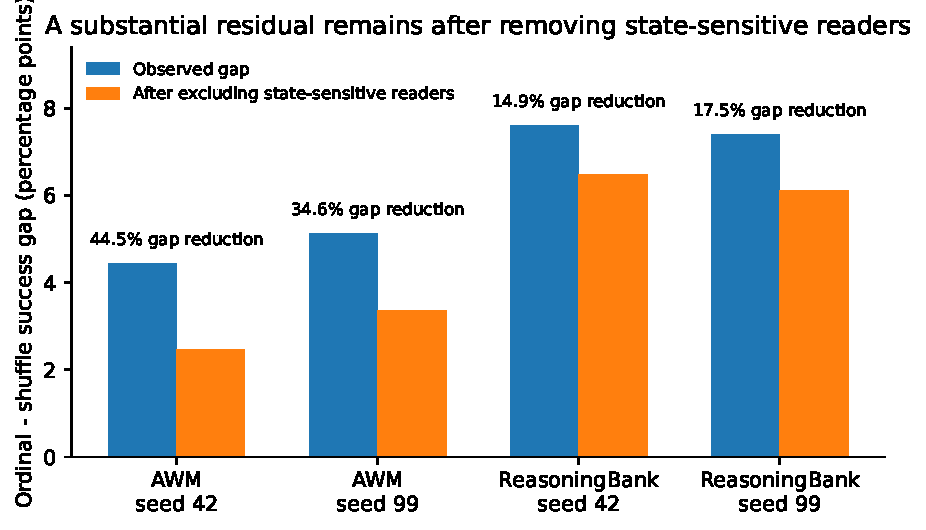
\includegraphics[width=0.98\linewidth]{figures/fig4_gap_sensitivity.pdf}
\caption{Observed task-order gap before and after excluding preregistered state-sensitive readers. Mutable-reference tasks account for a material fraction of the measured gap, especially for AWM.}
\label{fig:gap}
\end{figure}

The released task-order effect therefore contains an identifiable environment-sensitive component. After state-sensitive readers are removed, AWM retains 2.46--3.36 percentage points of order sensitivity. ReasoningBank retains more than six percentage points. The residual defines the effect that a state-isolated rerun can attribute more directly to self-improvement history.
